\documentclass[11pt]{article}

\usepackage[utf8]{inputenc}
\usepackage{amsmath}
\usepackage{amssymb}
\usepackage{amsthm}
\usepackage{geometry}
\usepackage[colorlinks=true, linkcolor=blue, citecolor=blue, urlcolor=blue]{hyperref}
\usepackage{mathrsfs}
\usepackage{mathtools}
\usepackage{tikz}

\geometry{letterpaper, margin=1in}
\renewcommand{\qedsymbol}{$\blacksquare$}

\title{\textbf{Advanced Mathematical Logic, Proof Techniques, and Quantitative Modeling}}
\author{Tashfeen Omran}
\date{October 2026}

\begin{document}

\maketitle

\tableofcontents
\newpage

\section{Concept Checklist \& Question Mapping}
\label{sec:checklist_start}
The following checklist details the theoretical concepts, logical structures, and proof techniques extracted from the source material. Every concept is rigorously tested in the accompanying problem set.

\begin{itemize}
    \item \textbf{C1: Direct Proof (Number Theory)} - Algebraic substitution and integer closure. (Tested in Q1)
    \item \textbf{C2: Proof by Contrapositive (Number Theory)} - Negating conclusions to form workable assumptions. (Tested in Q2, Q24)
    \item \textbf{C3: Proof by Contradiction (Number Theory)} - Deducing logical impossibilities ($C$). (Tested in Q3, Q23)
    \item \textbf{C4: Direct Proof (Real Analysis)} - Order axioms and inequality manipulation. (Tested in Q4, Q25)
    \item \textbf{C5: Proof by Contrapositive (Real Analysis)} - Reversing inequality directions. (Tested in Q5)
    \item \textbf{C6: Proof by Contradiction (Real Analysis)} - Bounding arguments and non-existence. (Tested in Q6, Q26)
    \item \textbf{C7: Biconditional Proofs ($P \iff Q$)} - Proving both forward and backward implications. (Tested in Q7, Q8, Q27)
    \item \textbf{C8: Set-Theoretic Foundations} - Isomorphisms between logic and sets ($A \subseteq B \equiv P \implies Q$). (Tested in Q9, Q10, Q30)
    \item \textbf{C9: The ``Isolate the Variable'' Trick} - Avoiding fractions to maintain integer closure $\mathbb{Z}$. (Tested in Q11)
    \item \textbf{C10: Exploiting Domain Constraints} - Using $\mathbb{R}^+$ to divide without flipping inequalities. (Tested in Q12)
    \item \textbf{C11: Transitivity of Inequalities} - Constructing intermediate terms. (Tested in Q13)
    \item \textbf{C12: Logical Equivalences} - De Morgan's Laws and implication negations. (Tested in Q14)
    \item \textbf{C13: Abstract Modeling (Quant Finance)} - Arbitrage Pricing Theory and Binomial Models. (Tested in Q15, Q16, Q28)
    \item \textbf{C14: Abstract Modeling (Machine Learning)} - PAC learning bounds and generalization error. (Tested in Q17, Q29)
    \item \textbf{C15: Diagnostic Testing (Find the Flaw)} - Affirming the Consequent, Denying the Antecedent, Division by Zero Probability, Incomplete Cases, Circular Reasoning. (Tested in Q18, Q19, Q20, Q21, Q22)
\end{itemize}

\newpage

\section{Problem Set}
\label{sec:problems}

\begin{enumerate}
    \item \textbf{[C1]} Prove by direct proof: If $n$ is an odd integer, then $5n + 7$ is an even integer.
    \item \textbf{[C2]} Prove by contrapositive: If $3n - 4$ is an even integer, then $n$ is an even integer.
    \item \textbf{[C3]} Prove by contradiction: There is no integer $n$ such that $6n + 1$ is a multiple of 3.
    \item \textbf{[C4]} Let $x \in \mathbb{R}^+$. Prove by direct proof: If $x > 4$, then $x^2 - 2x > 8$.
    \item \textbf{[C5]} Let $x \in \mathbb{R}^+$. Prove by contrapositive: If $x^3 + 2x < 0$, then $x < 0$.
    \item \textbf{[C6]} Prove by contradiction: There is no largest negative rational number.
    \item \textbf{[C7]} Prove the biconditional statement: For any integer $n$, $n^2$ is a multiple of 3 if and only if $n$ is a multiple of 3.
    \item \textbf{[C7]} Let $x \in \mathbb{R}^+$. Prove the biconditional statement: $x + \frac{9}{x} \ge 6 \iff (x-3)^2 \ge 0$.
    \item \textbf{[C8]} Prove set-theoretically that $A \subseteq B \implies A \cap B^c = \emptyset$.
    \item \textbf{[C8]} Prove set-theoretically that $(A \cup B)^c = A^c \cap B^c$.
    \item \textbf{[C9]} Prove that if $9n - 5$ is even, then $n$ is odd. You must use the ``Isolate the Variable'' trick to maintain integer closure and avoid fractions.
    \item \textbf{[C10]} Let $x \in \mathbb{R}^+$. Prove that if $x - \frac{5}{x} > 4$, then $x > 5$. Explicitly state where the domain constraint is exploited.
    \item \textbf{[C11]} Let $a, b, c \in \mathbb{R}^+$. Prove that if $a < b$ and $b < c$, then $a^2 < c^2$ using the transitivity of inequalities.
    \item \textbf{[C12]} Establish the logical equivalence of $P \implies (Q \lor R)$ and $(P \land \sim Q) \implies R$.
    \item \textbf{[C13]} In a one-period binomial model, let $S_0 = 100$, $u = 1.2$, $d = 0.9$, and the risk-free rate $r = 0.05$. Prove by contradiction that this market is arbitrage-free.
    \item \textbf{[C13]} In a one-period binomial model, let $S_0 = 50$, $u = 1.1$, $d = 0.8$, and $r = 0.15$. Prove by contradiction that an arbitrage opportunity exists, and construct the exact portfolio that exploits it.
    \item \textbf{[C14]} In Statistical Learning Theory, the probability of the empirical risk $R_E$ diverging from the true risk $R_T$ is bounded by $\mathbb{P}(|R_E - R_T| > \epsilon) \le 2 \exp(-2N\epsilon^2)$. Prove by contrapositive that if $\mathbb{P}(|R_E - R_T| > \epsilon) > \delta$, then the sample size $N$ is strictly bounded above by $\frac{\ln(2/\delta)}{2\epsilon^2}$.
    \item \textbf{[C15]} Find the flaw in the following proof: \textit{Statement: If $x > 0$, then $x^2 > 0$. Proof: Assume $x^2 > 0$. Since $x^2 = 4 > 0$, it follows that $x = 2 > 0$. Thus the statement is true.}
    \item \textbf{[C15]} Find the flaw in the following proof: \textit{Statement: If $n$ is a multiple of 4, then $n$ is even. Proof: Assume $n$ is not a multiple of 4. Then $n$ is odd. Since $n$ is odd, it is not even. This proves the inverse, which is logically equivalent.}
    \item \textbf{[C15]} Find the flaw in the following proof: \textit{Statement: If $\mathbb{P}(A|B) = \mathbb{P}(A)$, then $A$ and $B$ are independent. Proof: By definition, $\mathbb{P}(A|B) = \frac{\mathbb{P}(A \cap B)}{\mathbb{P}(B)}$. Setting this equal to $\mathbb{P}(A)$ yields $\mathbb{P}(A \cap B) = \mathbb{P}(A)\mathbb{P}(B)$, proving independence.}
    \item \textbf{[C15]} Find the flaw in the following proof: \textit{Statement: If $n^2$ is divisible by 6, then $n$ is divisible by 6. Proof: Assume $n$ is not divisible by 6. Then $n = 6k+1$. Squaring yields $n^2 = 36k^2 + 12k + 1 = 6(6k^2 + 2k) + 1$, which is not divisible by 6. This proves the contrapositive.}
    \item \textbf{[C15]} Find the flaw in the following proof: \textit{Statement: For $x, y \in \mathbb{R}$, $\sqrt{x^2 + y^2} \le |x| + |y|$. Proof: Squaring both sides gives $x^2 + y^2 \le x^2 + 2|xy| + y^2$. Subtracting $x^2 + y^2$ gives $0 \le 2|xy|$, which is always true. Therefore, the original statement is true.}
    \item \textbf{[C3]} Prove by contradiction that $\sqrt{5}$ is irrational.
    \item \textbf{[C2]} Prove by contrapositive that if $ab$ is even, then $a$ is even or $b$ is even.
    \item \textbf{[C4]} Prove directly that for any $x, y \in \mathbb{R}^+$, $\frac{x+y}{2} \ge \sqrt{xy}$.
    \item \textbf{[C6]} Prove by contradiction that the multiplicative inverse of a non-zero real number $x$ is unique.
    \item \textbf{[C7]} Prove the biconditional set-theoretic statement: $A \setminus B = A \iff A \cap B = \emptyset$.
    \item \textbf{[C13]} Prove by contradiction that in a binomial model, if $d \ge 1+r$, an arbitrage opportunity exists.
    \item \textbf{[C14]} Prove that if $A$ and $B$ are independent events in a probability space $\Omega$ and $A \subseteq B$, then either $\mathbb{P}(A) = 0$ or $\mathbb{P}(B) = 1$.
    \item \textbf{[C8]} Prove that the logical statement $\sim(P \implies Q)$ is set-theoretically isomorphic to $A \cap B^c$, and use this to prove that $\sim(P \implies Q) \implies P$ is a tautology.
\end{enumerate}

\newpage

\section{Detailed Solutions}
\label{sec:solutions}

\begin{enumerate}
    % Solution 1
    \item \textbf{Direct Proof.} Let $n$ be an arbitrary odd integer. By definition, there exists an integer $k \in \mathbb{Z}$ such that $n = 2k + 1$. Substituting this into the expression:
    \begin{align*}
        5n + 7 &= 5(2k + 1) + 7 \\
               &= 10k + 5 + 7 \\
               &= 10k + 12 \\
               &= 2(5k + 6)
    \end{align*}
    Since $k \in \mathbb{Z}$, the expression $m = 5k + 6$ is an integer due to the closure of integers under addition and multiplication. Thus, $5n + 7 = 2m$, which is the definition of an even integer.
    \begin{proof}\renewcommand{\qedsymbol}{$\blacksquare$}\end{proof}

    % Solution 2
    \item \textbf{Proof by Contrapositive.} We aim to prove: If $n$ is an odd integer, then $3n - 4$ is an odd integer. Assume $n$ is odd. By definition, $n = 2k + 1$ for some $k \in \mathbb{Z}$. Substituting this into the expression:
    \begin{align*}
        3n - 4 &= 3(2k + 1) - 4 \\
               &= 6k + 3 - 4 \\
               &= 6k - 1 \\
               &= 6k - 2 + 1 \\
               &= 2(3k - 1) + 1
    \end{align*}
    Let $m = 3k - 1$. Since $k \in \mathbb{Z}$, $m \in \mathbb{Z}$. Thus, $3n - 4 = 2m + 1$, which means $3n - 4$ is odd. By proving the contrapositive, the original statement holds.
    \begin{proof}\renewcommand{\qedsymbol}{$\blacksquare$}\end{proof}

    % Solution 3
    \item \textbf{Proof by Contradiction.} Assume, to the contrary, that there exists an integer $n$ such that $6n + 1$ is a multiple of 3. By definition, there exists an integer $k \in \mathbb{Z}$ such that $6n + 1 = 3k$. Rearranging the equation yields:
    \begin{align*}
        1 &= 3k - 6n \\
        1 &= 3(k - 2n)
    \end{align*}
    Since $k, n \in \mathbb{Z}$, let $m = k - 2n \in \mathbb{Z}$. This implies $1 = 3m$. Dividing by 3 gives $m = \frac{1}{3}$. However, $m$ must be an integer, and $\frac{1}{3} \notin \mathbb{Z}$. This is a contradiction. Therefore, no such integer $n$ exists.
    \begin{proof}\renewcommand{\qedsymbol}{$\blacksquare$}\end{proof}

    % Solution 4
    \item \textbf{Direct Proof.} Let $x \in \mathbb{R}^+$. Assume $x > 4$. Since $x > 0$, we can multiply both sides of the inequality by $x$ without changing the direction:
    \[ x^2 > 4x \]
    We can also multiply the original assumption $x > 4$ by 2 to get $2x > 8$. Subtracting $2x$ from both sides of $x^2 > 4x$ yields:
    \[ x^2 - 2x > 2x \]
    Since $2x > 8$, by the transitivity of inequalities, we have:
    \[ x^2 - 2x > 8 \]
    \begin{proof}\renewcommand{\qedsymbol}{$\blacksquare$}\end{proof}

    % Solution 5
    \item \textbf{Proof by Contrapositive.} We aim to prove: If $x \ge 0$, then $x^3 + 2x \ge 0$. Assume $x \ge 0$. Since $x$ is non-negative, $x^2 \ge 0$. Multiplying by $x$ (which is non-negative) yields $x^3 \ge 0$. Furthermore, multiplying $x \ge 0$ by 2 yields $2x \ge 0$. Adding these two non-negative quantities gives:
    \[ x^3 + 2x \ge 0 \]
    This proves the contrapositive, establishing the truth of the original statement.
    \begin{proof}\renewcommand{\qedsymbol}{$\blacksquare$}\end{proof}

    % Solution 6
    \item \textbf{Proof by Contradiction.} Assume, to the contrary, that there exists a largest negative rational number, say $q$. Since $q$ is a negative rational, $q < 0$ and $q = \frac{a}{b}$ for some integers $a, b$ with $b \neq 0$. Consider the number $q' = \frac{q}{2}$. Since $q < 0$, dividing by 2 preserves the sign, so $q' < 0$. Furthermore, $q' = \frac{a}{2b}$, which is the ratio of two integers, so $q'$ is rational. Because $q < 0$, dividing by 2 yields a number closer to zero, meaning $q < \frac{q}{2} < 0$. Thus, $q < q'$. This means $q'$ is a negative rational number strictly greater than $q$, contradicting the assumption that $q$ is the largest negative rational number.
    \begin{proof}\renewcommand{\qedsymbol}{$\blacksquare$}\end{proof}

    % Solution 7
    \item \textbf{Biconditional Proof.} We must prove both directions. \\
    \textit{Part 1 ($\impliedby$):} Assume $n$ is a multiple of 3. Then $n = 3k$ for $k \in \mathbb{Z}$. $n^2 = (3k)^2 = 9k^2 = 3(3k^2)$. Since $3k^2 \in \mathbb{Z}$, $n^2$ is a multiple of 3. \\
    \textit{Part 2 ($\implies$):} We prove this by contrapositive. Assume $n$ is not a multiple of 3. Then $n = 3k + 1$ or $n = 3k + 2$. \\
    Case 1: $n = 3k + 1 \implies n^2 = 9k^2 + 6k + 1 = 3(3k^2 + 2k) + 1$, not a multiple of 3. \\
    Case 2: $n = 3k + 2 \implies n^2 = 9k^2 + 12k + 4 = 3(3k^2 + 4k + 1) + 1$, not a multiple of 3. \\
    Since both directions hold, the biconditional is true.
    \begin{proof}\renewcommand{\qedsymbol}{$\blacksquare$}\end{proof}

    % Solution 8
    \item \textbf{Biconditional Proof.} Let $x \in \mathbb{R}^+$. \\
    \textit{Part 1 ($\implies$):} Assume $x + \frac{9}{x} \ge 6$. Since $x > 0$, multiplying by $x$ preserves the inequality: $x^2 + 9 \ge 6x$. Subtracting $6x$ yields $x^2 - 6x + 9 \ge 0$. Factoring gives $(x-3)^2 \ge 0$. \\
    \textit{Part 2 ($\impliedby$):} Assume $(x-3)^2 \ge 0$. Expanding yields $x^2 - 6x + 9 \ge 0$. Adding $6x$ gives $x^2 + 9 \ge 6x$. Since $x \in \mathbb{R}^+$, $x > 0$, so we can divide by $x$ without flipping the inequality: $x + \frac{9}{x} \ge 6$.
    \begin{proof}\renewcommand{\qedsymbol}{$\blacksquare$}\end{proof}

    % Solution 9
    \item \textbf{Direct Proof.} Assume $A \subseteq B$. By definition, for all $x$, if $x \in A$, then $x \in B$. We want to show $A \cap B^c = \emptyset$. Assume, for the sake of contradiction, that $A \cap B^c \neq \emptyset$. Then there exists an element $x \in A \cap B^c$. This implies $x \in A$ and $x \in B^c$. Since $x \in B^c$, $x \notin B$. However, since $x \in A$ and $A \subseteq B$, it must be that $x \in B$. This is a contradiction ($x \in B \land x \notin B$). Therefore, $A \cap B^c = \emptyset$.
    \begin{proof}\renewcommand{\qedsymbol}{$\blacksquare$}\end{proof}

    % Solution 10
    \item \textbf{Set-Theoretic Proof.} We must show mutual inclusion. \\
    \textit{Part 1: $(A \cup B)^c \subseteq A^c \cap B^c$.} Let $x \in (A \cup B)^c$. By definition, $x \notin (A \cup B)$. This means it is false that $x \in A$ or $x \in B$. By De Morgan's Laws for logic, $x \notin A$ and $x \notin B$. Thus, $x \in A^c$ and $x \in B^c$, which implies $x \in A^c \cap B^c$. \\
    \textit{Part 2: $A^c \cap B^c \subseteq (A \cup B)^c$.} Let $x \in A^c \cap B^c$. Then $x \in A^c$ and $x \in B^c$, meaning $x \notin A$ and $x \notin B$. Therefore, $x$ cannot be in their union, so $x \notin (A \cup B)$, which means $x \in (A \cup B)^c$.
    \begin{proof}\renewcommand{\qedsymbol}{$\blacksquare$}\end{proof}

    % Solution 11
    \item \textbf{Proof by Contrapositive.} We aim to prove: If $n$ is even, then $9n - 5$ is odd. Assume $n$ is even. Then $n = 2k$ for some $k \in \mathbb{Z}$. Substituting this into the expression:
    \begin{align*}
        9n - 5 &= 9(2k) - 5 \\
               &= 18k - 5 \\
               &= 18k - 6 + 1 \\
               &= 2(9k - 3) + 1
    \end{align*}
    Let $m = 9k - 3 \in \mathbb{Z}$. Then $9n - 5 = 2m + 1$, which is odd. \\
    \textit{Alternative (Direct Proof with Isolate the Variable Trick):} Assume $9n - 5$ is even. Then $9n - 5 = 2k$. Adding 5 gives $9n = 2k + 5$. To isolate $n$ without fractions, subtract $8n$ from both sides:
    \begin{align*}
        9n - 8n &= 2k + 5 - 8n \\
        n &= 2k - 8n + 4 + 1 \\
        n &= 2(k - 4n + 2) + 1
    \end{align*}
    Since $k, n \in \mathbb{Z}$, $m = k - 4n + 2 \in \mathbb{Z}$. Thus $n = 2m + 1$, proving $n$ is odd.
    \begin{proof}\renewcommand{\qedsymbol}{$\blacksquare$}\end{proof}

    % Solution 12
    \item \textbf{Direct Proof.} Let $x \in \mathbb{R}^+$. Assume $x - \frac{5}{x} > 4$. Since $x > 0$ (exploiting the domain constraint), we can multiply both sides by $x$ without reversing the inequality:
    \[ x^2 - 5 > 4x \]
    Subtracting $4x$ yields $x^2 - 4x - 5 > 0$. Factoring the quadratic gives:
    \[ (x - 5)(x + 1) > 0 \]
    Since $x \in \mathbb{R}^+$, we know $x > 0$, which strictly implies $x + 1 > 1 > 0$. Because the factor $(x + 1)$ is strictly positive, we can divide both sides of the inequality by $(x + 1)$ without reversing the inequality sign (exploiting the domain constraint again):
    \[ x - 5 > 0 \implies x > 5 \]
    \begin{proof}\renewcommand{\qedsymbol}{$\blacksquare$}\end{proof}

    % Solution 13
    \item \textbf{Direct Proof.} Let $a, b, c \in \mathbb{R}^+$. Assume $a < b$ and $b < c$. Since $a, b > 0$, multiplying $a < b$ by $a$ gives $a^2 < ab$. Multiplying $a < b$ by $b$ gives $ab < b^2$. By transitivity, $a^2 < b^2$. Similarly, since $b, c > 0$, multiplying $b < c$ by $b$ gives $b^2 < bc$, and multiplying by $c$ gives $bc < c^2$. By transitivity, $b^2 < c^2$. Applying transitivity one final time to $a^2 < b^2$ and $b^2 < c^2$ yields $a^2 < c^2$.
    \begin{proof}\renewcommand{\qedsymbol}{$\blacksquare$}\end{proof}

    % Solution 14
    \item \textbf{Logical Equivalence Proof.} We use standard logical equivalences.
    \begin{align*}
        P \implies (Q \lor R) &\equiv \sim P \lor (Q \lor R) \quad \text{(Negation of Implication)} \\
                              &\equiv (\sim P \lor Q) \lor R \quad \text{(Associativity of Disjunction)} \\
                              &\equiv \sim(P \land \sim Q) \lor R \quad \text{(De Morgan's Law)} \\
                              &\equiv (P \land \sim Q) \implies R \quad \text{(Negation of Implication)}
    \end{align*}
    Thus, the two statements are logically isomorphic.
    \begin{proof}\renewcommand{\qedsymbol}{$\blacksquare$}\end{proof}

    % Solution 15
    \item \textbf{Proof by Contradiction.} Assume the market admits an arbitrage opportunity. This means there exists a portfolio with initial cost $X_0 = 0$, such that $X_1(\omega) \ge 0$ for all $\omega \in \{u, d\}$ and $\mathbb{P}(X_1 > 0) > 0$. Let the portfolio consist of $\Delta$ shares of stock and $B$ dollars in the risk-free bank account.
    \[ X_0 = \Delta S_0 + B = 0 \implies B = -\Delta S_0 \]
    At $t=1$, the portfolio value is $X_1(\omega) = \Delta S_1(\omega) + B(1+r) = \Delta(S_1(\omega) - S_0(1+r))$.
    Evaluating in both states:
    \begin{align*}
        X_1(u) &= \Delta S_0(u - (1+r)) = \Delta(100)(1.2 - 1.05) = 15\Delta \\
        X_1(d) &= \Delta S_0(d - (1+r)) = \Delta(100)(0.9 - 1.05) = -15\Delta
    \end{align*}
    For $X_1 \ge 0$ in all states, we need $15\Delta \ge 0 \implies \Delta \ge 0$ and $-15\Delta \ge 0 \implies \Delta \le 0$. The only solution is $\Delta = 0$. If $\Delta = 0$, then $X_1(u) = 0$ and $X_1(d) = 0$, which contradicts the requirement that $\mathbb{P}(X_1 > 0) > 0$. Thus, no arbitrage exists.
    \begin{proof}\renewcommand{\qedsymbol}{$\blacksquare$}\end{proof}

    % Solution 16
    \item \textbf{Proof by Contradiction.} Assume the market is arbitrage-free. We are given $u = 1.1$, $d = 0.8$, and $1+r = 1.15$. Notice that $d < u < 1+r$. We construct a portfolio by shorting 1 share of stock ($\Delta = -1$) and investing the proceeds in the bank ($B = S_0 = 50$). The initial cost is $X_0 = -50 + 50 = 0$. At $t=1$:
    \begin{align*}
        X_1(u) &= -S_0 u + S_0(1+r) = 50(1.15 - 1.1) = 50(0.05) = 2.5 \\
        X_1(d) &= -S_0 d + S_0(1+r) = 50(1.15 - 0.8) = 50(0.35) = 17.5
    \end{align*}
    Since $X_1(u) > 0$ and $X_1(d) > 0$, $X_1 \ge 0$ strictly, meaning $\mathbb{P}(X_1 > 0) = 1$. This portfolio requires zero initial investment and guarantees a strictly positive profit. This is an arbitrage opportunity, contradicting our assumption that the market is arbitrage-free.
    \begin{proof}\renewcommand{\qedsymbol}{$\blacksquare$}\end{proof}

    % Solution 17
    \item \textbf{Proof by Contrapositive.} The original statement is: If $N > \frac{\ln(2/\delta)}{2\epsilon^2}$, then $\mathbb{P}(|R_E - R_T| > \epsilon) \le \delta$. We assume the negation of the conclusion: $\mathbb{P}(|R_E - R_T| > \epsilon) > \delta$. We are given the fundamental PAC bound: $\mathbb{P}(|R_E - R_T| > \epsilon) \le 2 \exp(-2N\epsilon^2)$. By transitivity of inequalities:
    \[ \delta < 2 \exp(-2N\epsilon^2) \]
    Dividing by 2 (since $2 > 0$):
    \[ \frac{\delta}{2} < \exp(-2N\epsilon^2) \]
    Taking the natural logarithm of both sides (since $\ln(x)$ is strictly increasing for $x > 0$):
    \[ \ln\left(\frac{\delta}{2}\right) < -2N\epsilon^2 \]
    Using the property $\ln(a/b) = -\ln(b/a)$, we have $-\ln\left(\frac{2}{\delta}\right) < -2N\epsilon^2$. Dividing by $-2\epsilon^2$ (which is negative, so we flip the inequality):
    \[ \frac{\ln(2/\delta)}{2\epsilon^2} > N \implies N < \frac{\ln(2/\delta)}{2\epsilon^2} \]
    This proves the contrapositive.
    \begin{proof}\renewcommand{\qedsymbol}{$\blacksquare$}\end{proof}

    % Solution 18
    \item \textbf{Flaw Identification:} The proof commits the logical fallacy of \textbf{Affirming the Consequent}. It assumes the conclusion ($x^2 > 0$) to prove the hypothesis ($x > 0$). Furthermore, the deduction $x^2 = 4 \implies x = 2$ is algebraically incomplete, as $x$ could be $-2$, which would make $x > 0$ false. A correct direct proof must start with $x > 0$ and multiply both sides by $x$ to get $x^2 > 0$.

    % Solution 19
    \item \textbf{Flaw Identification:} The proof commits the logical fallacy of \textbf{Denying the Antecedent}. It assumes the negation of the hypothesis ($\sim P$) to deduce the negation of the conclusion ($\sim Q$). This proves the inverse ($\sim P \implies \sim Q$), which is logically equivalent to the converse, not the original statement. To prove the statement, one must assume $n = 4k$ and deduce $n = 2(2k)$.

    % Solution 20
    \item \textbf{Flaw Identification:} The proof commits a \textbf{Division by Zero Probability} error. The definition $\mathbb{P}(A|B) = \frac{\mathbb{P}(A \cap B)}{\mathbb{P}(B)}$ is only valid under the strict domain constraint that $\mathbb{P}(B) > 0$. The proof fails to establish this prerequisite. If $\mathbb{P}(B) = 0$, the conditional probability is undefined in standard Kolmogorov axioms, making the algebraic manipulation invalid.

    % Solution 21
    \item \textbf{Flaw Identification:} The proof suffers from \textbf{Incomplete Cases}. The negation of ``$n$ is divisible by 6'' is not simply $n = 6k+1$. By the Division Algorithm, if $n$ is not divisible by 6, it could be $6k+1, 6k+2, 6k+3, 6k+4,$ or $6k+5$. The proof fails to check the other four cases. (In fact, if $n = 6k+2$, $n^2 = 36k^2 + 24k + 4$, which is not divisible by 6, but if $n=6k+3$, $n^2 = 36k^2 + 36k + 9$, still not divisible. However, the logical structure of the proof is invalid without exhaustive case analysis).

    % Solution 22
    \item \textbf{Flaw Identification:} The proof commits \textbf{Circular Reasoning (Begging the Question)}. It assumes the inequality it is trying to prove ($\sqrt{x^2 + y^2} \le |x| + |y|$) and algebraically manipulates it to reach a known tautology ($0 \le 2|xy|$). A valid proof must start from the tautology $0 \le 2|xy|$ and work backward to the desired conclusion.

    % Solution 23
    \item \textbf{Proof by Contradiction.} Assume $\sqrt{5}$ is rational. Then there exist integers $a, b$ with $b \neq 0$ such that $\sqrt{5} = \frac{a}{b}$, and $\gcd(a,b) = 1$ (the fraction is in simplest form). Squaring both sides yields $5 = \frac{a^2}{b^2}$, so $a^2 = 5b^2$. This implies $a^2$ is a multiple of 5. Since 5 is prime, $a$ must also be a multiple of 5. Let $a = 5k$ for some $k \in \mathbb{Z}$. Substituting this back gives $(5k)^2 = 5b^2 \implies 25k^2 = 5b^2 \implies 5k^2 = b^2$. This implies $b^2$ is a multiple of 5, and thus $b$ is a multiple of 5. If both $a$ and $b$ are multiples of 5, then $\gcd(a,b) \ge 5$, which contradicts our assumption that $\gcd(a,b) = 1$. Thus, $\sqrt{5}$ is irrational.
    \begin{proof}\renewcommand{\qedsymbol}{$\blacksquare$}\end{proof}

    % Solution 24
    \item \textbf{Proof by Contrapositive.} The statement is $P \implies (Q \lor R)$. The contrapositive is $\sim(Q \lor R) \implies \sim P$. By De Morgan's Laws, this is $(\sim Q \land \sim R) \implies \sim P$. Thus, we assume $a$ is odd AND $b$ is odd. By definition, $a = 2k+1$ and $b = 2m+1$ for $k, m \in \mathbb{Z}$.
    \begin{align*}
        ab &= (2k+1)(2m+1) \\
           &= 4km + 2k + 2m + 1 \\
           &= 2(2km + k + m) + 1
    \end{align*}
    Since $k, m \in \mathbb{Z}$, let $j = 2km + k + m \in \mathbb{Z}$. Then $ab = 2j + 1$, which means $ab$ is odd. This proves the contrapositive.
    \begin{proof}\renewcommand{\qedsymbol}{$\blacksquare$}\end{proof}

    % Solution 25
    \item \textbf{Direct Proof.} Let $x, y \in \mathbb{R}^+$. We know that the square of any real number is non-negative. Consider the real number $(\sqrt{x} - \sqrt{y})$.
    \[ (\sqrt{x} - \sqrt{y})^2 \ge 0 \]
    Expanding the square yields:
    \[ x - 2\sqrt{xy} + y \ge 0 \]
    Adding $2\sqrt{xy}$ to both sides gives:
    \[ x + y \ge 2\sqrt{xy} \]
    Dividing by 2 yields the AM-GM inequality:
    \[ \frac{x+y}{2} \ge \sqrt{xy} \]
    \begin{proof}\renewcommand{\qedsymbol}{$\blacksquare$}\end{proof}

    % Solution 26
    \item \textbf{Proof by Contradiction.} Let $x \in \mathbb{R}$ with $x \neq 0$. Assume, to the contrary, that $x$ has two distinct multiplicative inverses, say $y$ and $z$, such that $y \neq z$. By the definition of a multiplicative inverse, $xy = 1$ and $xz = 1$. Consider the expression $y(xz)$. By associativity of multiplication:
    \[ y(xz) = (yx)z \]
    Since multiplication is commutative, $yx = xy = 1$. Substituting the known values:
    \[ y(1) = (1)z \implies y = z \]
    This contradicts our initial assumption that $y \neq z$. Therefore, the multiplicative inverse must be unique.
    \begin{proof}\renewcommand{\qedsymbol}{$\blacksquare$}\end{proof}

    % Solution 27
    \item \textbf{Biconditional Proof.} \\
    \textit{Part 1 ($\implies$):} Assume $A \setminus B = A$. We want to show $A \cap B = \emptyset$. Assume for contradiction that $A \cap B \neq \emptyset$. Then $\exists x \in A \cap B$, meaning $x \in A$ and $x \in B$. Since $x \in B$, $x \notin A \setminus B$. But $A \setminus B = A$, so $x \notin A$. This contradicts $x \in A$. Thus, $A \cap B = \emptyset$. \\
    \textit{Part 2 ($\impliedby$):} Assume $A \cap B = \emptyset$. We want to show $A \setminus B = A$. Let $x \in A$. Since $A \cap B = \emptyset$, $x \notin B$. Thus $x \in A$ and $x \notin B$, which means $x \in A \setminus B$. So $A \subseteq A \setminus B$. Now let $y \in A \setminus B$. By definition, $y \in A$ and $y \notin B$. Thus $y \in A$, so $A \setminus B \subseteq A$. Mutual inclusion proves $A \setminus B = A$.
    \begin{proof}\renewcommand{\qedsymbol}{$\blacksquare$}\end{proof}

    % Solution 28
    \item \textbf{Proof by Contradiction.} Assume the market is arbitrage-free, but $d \ge 1+r$. We construct a portfolio by shorting the bank ($B = -S_0$) and buying 1 share of stock ($\Delta = 1$). Initial cost $X_0 = S_0 - S_0 = 0$. At $t=1$:
    \begin{align*}
        X_1(u) &= uS_0 - S_0(1+r) = S_0(u - (1+r)) \\
        X_1(d) &= dS_0 - S_0(1+r) = S_0(d - (1+r))
    \end{align*}
    Since $d < u$ and $d \ge 1+r$, it strictly follows that $u > 1+r$. Thus $X_1(u) > 0$. Since $d \ge 1+r$, $X_1(d) \ge 0$. The portfolio has $X_0 = 0$, $X_1 \ge 0$ in all states, and $\mathbb{P}(X_1 > 0) > 0$ (since the up-state has positive probability). This is an arbitrage opportunity, contradicting the assumption.
    \begin{proof}\renewcommand{\qedsymbol}{$\blacksquare$}\end{proof}

    % Solution 29
    \item \textbf{Direct Proof.} Let $A$ and $B$ be independent events, meaning $\mathbb{P}(A \cap B) = \mathbb{P}(A)\mathbb{P}(B)$. We are given $A \subseteq B$. Set-theoretically, if $A \subseteq B$, then $A \cap B = A$. Therefore, $\mathbb{P}(A \cap B) = \mathbb{P}(A)$. Substituting this into the independence equation yields:
    \[ \mathbb{P}(A) = \mathbb{P}(A)\mathbb{P}(B) \]
    Subtracting $\mathbb{P}(A)\mathbb{P}(B)$ from both sides gives:
    \[ \mathbb{P}(A) - \mathbb{P}(A)\mathbb{P}(B) = 0 \]
    Factoring out $\mathbb{P}(A)$:
    \[ \mathbb{P}(A)(1 - \mathbb{P}(B)) = 0 \]
    By the zero-product property of real numbers, either $\mathbb{P}(A) = 0$ or $1 - \mathbb{P}(B) = 0 \implies \mathbb{P}(B) = 1$.
    \begin{proof}\renewcommand{\qedsymbol}{$\blacksquare$}\end{proof}

    % Solution 30
    \item \textbf{Set-Theoretic Isomorphism Proof.} First, we translate $\sim(P \implies Q)$. By the Negation of Implication equivalence, $\sim(P \implies Q) \equiv P \land \sim Q$. Let $A$ be the truth set of $P$ and $B$ be the truth set of $Q$. The logical conjunction ($\land$) maps to set intersection ($\cap$), and logical negation ($\sim$) maps to set complement ($^c$). Thus, $P \land \sim Q$ is isomorphic to $A \cap B^c$. 
    
    To prove $\sim(P \implies Q) \implies P$ is a tautology, we map it to sets. The implication $X \implies Y$ is isomorphic to $X \subseteq Y$. We must show $(A \cap B^c) \subseteq A$. Let $x \in A \cap B^c$. By definition of intersection, $x \in A$ and $x \in B^c$. Since $x \in A$, the condition for subset inclusion is met. Because $(A \cap B^c) \subseteq A$ is universally true for all sets, the isomorphic logical statement is a tautology.
    
    \begin{center}
    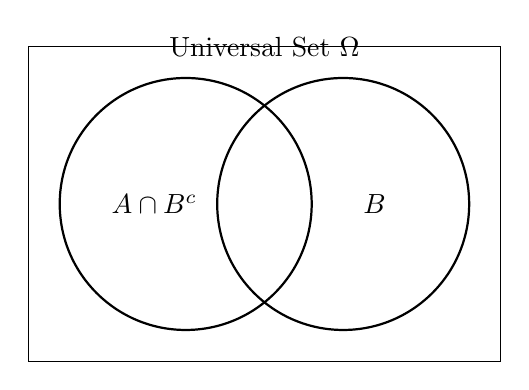
\begin{tikzpicture}[scale=0.8]
        % Venn Diagram for A \cap B^c
        \draw[thick] (0,0) circle (2cm);
        \draw[thick] (2.5,0) circle (2cm);
        \node at (-0.5, 0) {$A \cap B^c$};
        \node at (3, 0) {$B$};
        \node at (1.25, 2.5) {Universal Set $\Omega$};
        \draw (-2.5,-2.5) rectangle (5,2.5);
    \end{tikzpicture}
    \end{center}
    \begin{proof}\renewcommand{\qedsymbol}{$\blacksquare$}\end{proof}

\end{enumerate}

\newpage

\section{Concept Checklist \& Question Mapping (Repeated)}
\label{sec:checklist_end}
\begin{itemize}
    \item \textbf{C1: Direct Proof (Number Theory)} - Algebraic substitution and integer closure. (Tested in Q1)
    \item \textbf{C2: Proof by Contrapositive (Number Theory)} - Negating conclusions to form workable assumptions. (Tested in Q2, Q24)
    \item \textbf{C3: Proof by Contradiction (Number Theory)} - Deducing logical impossibilities ($C$). (Tested in Q3, Q23)
    \item \textbf{C4: Direct Proof (Real Analysis)} - Order axioms and inequality manipulation. (Tested in Q4, Q25)
    \item \textbf{C5: Proof by Contrapositive (Real Analysis)} - Reversing inequality directions. (Tested in Q5)
    \item \textbf{C6: Proof by Contradiction (Real Analysis)} - Bounding arguments and non-existence. (Tested in Q6, Q26)
    \item \textbf{C7: Biconditional Proofs ($P \iff Q$)} - Proving both forward and backward implications. (Tested in Q7, Q8, Q27)
    \item \textbf{C8: Set-Theoretic Foundations} - Isomorphisms between logic and sets ($A \subseteq B \equiv P \implies Q$). (Tested in Q9, Q10, Q30)
    \item \textbf{C9: The ``Isolate the Variable'' Trick} - Avoiding fractions to maintain integer closure $\mathbb{Z}$. (Tested in Q11)
    \item \textbf{C10: Exploiting Domain Constraints} - Using $\mathbb{R}^+$ to divide without flipping inequalities. (Tested in Q12)
    \item \textbf{C11: Transitivity of Inequalities} - Constructing intermediate terms. (Tested in Q13)
    \item \textbf{C12: Logical Equivalences} - De Morgan's Laws and implication negations. (Tested in Q14)
    \item \textbf{C13: Abstract Modeling (Quant Finance)} - Arbitrage Pricing Theory and Binomial Models. (Tested in Q15, Q16, Q28)
    \item \textbf{C14: Abstract Modeling (Machine Learning)} - PAC learning bounds and generalization error. (Tested in Q17, Q29)
    \item \textbf{C15: Diagnostic Testing (Find the Flaw)} - Affirming the Consequent, Denying the Antecedent, Division by Zero Probability, Incomplete Cases, Circular Reasoning. (Tested in Q18, Q19, Q20, Q21, Q22)
\end{itemize}

\end{document}